\chapter{Capitolo 4: Algoritmi basati sulla distanza}
In questo capitolo vengono illustrati i principali algoritmi utilizzati per la costruzione degli alberi evolutivi. L'obiettivo è quello di trovare una soluzione al cosiddetto \textit{problema degli alberi basati sulla distanza}, ma prima è necessario introdurre alcuni concetti, tra cui la matrice delle distanze.

\section{Matrice delle distanze}
Dati due punti, $x$ e $y$, la \textit{distanza} può essere vista come loro "lontananza" in uno spazio $k$-dimensionale. Nella fattispecie è una funzione $d(x,y)$ che possiede le seguenti proprietà \cite{dataMiningInBioinformatics}:
\begin{enumerate}
	\item \textit{non negatività}:
	\[d(x,y)\geq 0\hspace{2em} \forall \: x,y\in R^k\]
	\item \textit{identità}:
	\[d(x,y)=0 \; \leftrightarrow \; x=y\]
	\item \textit{simmetria}:
	\[d(x,y)=d(y,x)\hspace{2em} \forall \: x,y\in R^k\]
	\item \textit{disuguaglianza triangolare}:
	\[d(x,y)\leq d(x,z)+d(y,z)\hspace{2em} \forall \: x,y,z\in R^k\]
\end{enumerate}
Date $n$ unità, calcolando la distanza per ogni coppia di elementi\footnote{Ci sono vari modi per calcolare la distanza tra due elementi, ad esempio attraverso la distanza Euclidea, quella di Manhattan, di Minkowski e così via.} si ottiene una \textit{matrice delle distanze $n \times n$}, definita nel seguente modo \cite{introductionbioinfalg}:
\[
D = \begin{pmatrix}
0 & d_{12} & d_{13} & \ldots & d_{1n} \\ 
d_{21} & 0 & d_{23} & \ldots & d_{2n} \\ 
d_{31} & d_{32} & 0 & \ldots & d_{3n} \\ 
\vdots & \vdots & \vdots & \ddots & \vdots \\ 
d_{n1} & d_{n2} & \ldots & \ldots & 0
\end{pmatrix}
\hspace{3em}dove\;d(x_i,x_j)=D_i,_j
\]
Poiché la matrice è costruita a partire dalle distanze, ne eredita le proprietà precedentemente elencate.
\newline
Ciascun valore $D_i,_j$ può assumere significati diversi in base al contesto, ad esempio può indicare il numero di simboli diversi tra i geni $i$ e $j$ nell'allineamento di sequenze di DNA\footnote{L'allineamento è il processo attraverso il quale si misura la similarità tra due o più sequenze.}, come mostrato nell'esempio sottostante:
\begin{figure}[h!]
	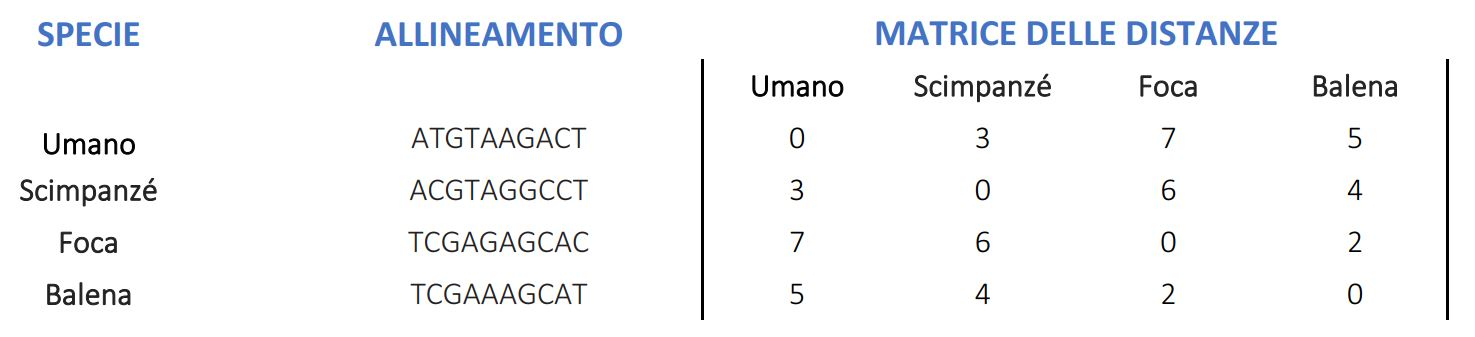
\includegraphics[width=\linewidth]{distance_matrix_example.jpg}
 	\caption{Esempio di matrice delle distanze.}
  	\label{fig:DistanceMatrix}
\end{figure}
\newline
Nella figura 5 è possibile notare che la sequenza di DNA della foca risulta molto più simile a quella della balena, in quanto la distanza è $2$, rispetto a quella dell'umano, con cui la distanza è $7$.
\newpage

\section{Problema degli alberi basati sulla distanza}
Gli algoritmi basati sulla distanza utilizzano la matrice delle distanze per costruire gli alberi evolutivi, dove le foglie corrispondono alle entità biologiche presenti nella matrice, mentre i nodi interni rappresentano gli antenati non noti. Per poter calcolare la distanza tra due foglie, e quindi conoscere quanto sono legate tra loro, è necessario associare un valore non negativo (peso) a ciascun arco e definire la lunghezza di un cammino in tale albero come la somma dei pesi degli archi che lo compongono. Si definisce, quindi, la \textit{distanza evolutiva} tra due entità biologiche corrispondenti alle foglie $i$ e $j$ di un albero $T$ come la lunghezza dell'unico cammino che le collega, ed è indicato come $d_i,_j(T)$ \cite{bioinfalganactivelearningapproachparttwo}. In altre parole è data dalla somma dei pesi degli archi che ci sono tra $i$ e $j$.
\newline
Si dice che un albero $T$ si \textit{adatta} ad una matrice delle distanze $D$ se per ogni coppia di foglie $i$ e $j$ si ha che $D_i,_j=d_i,_j(T)$, ovvero l'elemento nella riga $i$ e colonna $j$ è uguale alla lunghezza del cammino che collega le due foglie in $T$ (distanza evolutiva), in tal caso sia la matrice che l'albero vengono definiti \textit{additivi}. Qualora invece non esista un albero che si adatti alla matrice, allora tale matrice è detta \textit{non additiva} \cite{bioinfalganactivelearningapproachparttwo}.
\newline
Si riporta di seguito un esempio che mostra un albero che si adatta alla matrice delle distanze mostrata nella sezione precedente.
\begin{figure}[h!]
	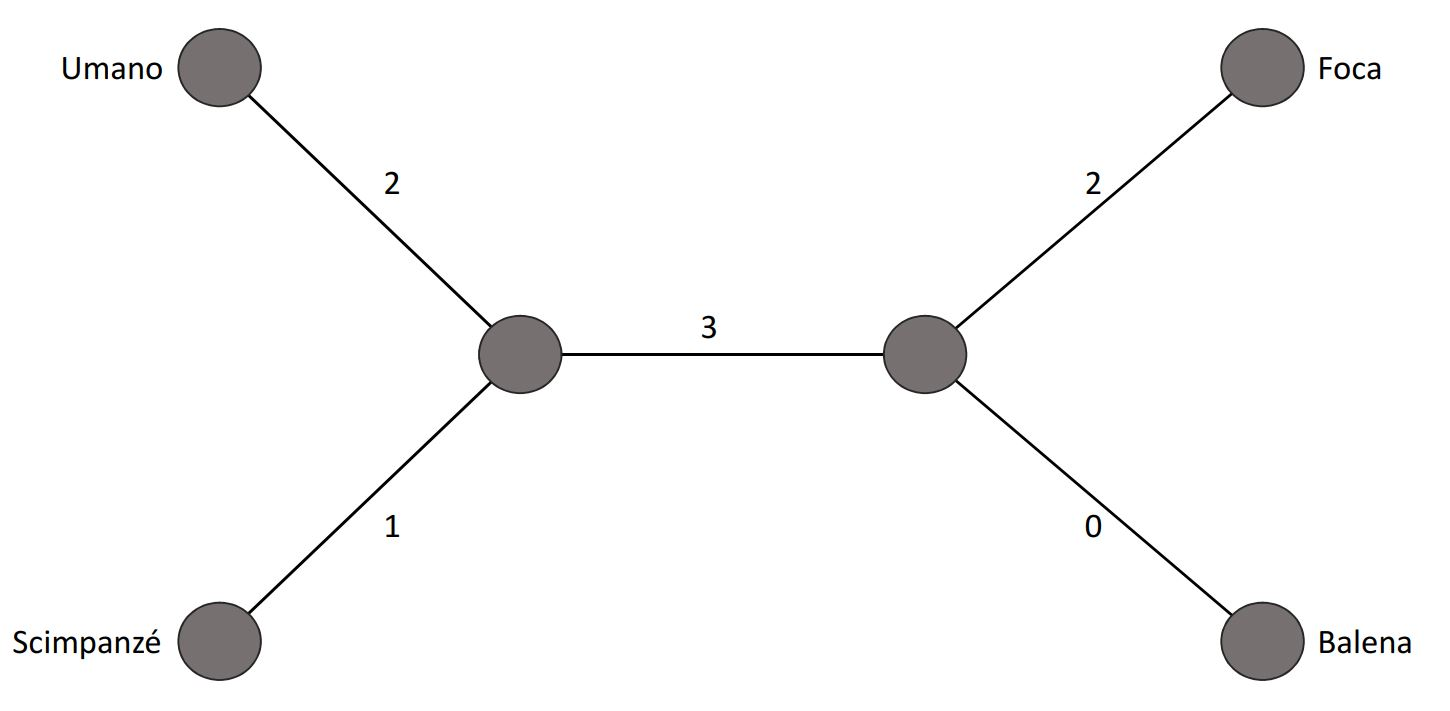
\includegraphics[width=\linewidth]{unrooted_tree_created_by_figure_5.jpg}
 	\caption{Albero evolutivo senza radice costruito a partire dalla matrice \textbf{additiva} della figura 5.}
  	\label{fig:EvolutionaryTreeExample}
\end{figure}
\newline
Ci possono essere più alberi che si adattano ad una matrice, quindi come si può scegliere l'albero giusto? Si nota che quello in figura 6 ha tutti i vertici di grado diverso da due e viene definito \textit{albero semplice}. 
\newpage
Una caratteristica importante è che per ogni matrice delle distanze additiva esiste un unico albero semplice che si adatta alla matrice stessa.
\newline
Adesso è possibile dare una definizione al problema accennato all'inizio del capitolo, mostrata di seguito.
\newline
\newline
\textbf{Problema degli alberi basati sulla distanza:}
\newline
\textit{Data in \textbf{input} una matrice delle distanze additiva restituire in \textbf{output} un albero evolutivo semplice.}

\newpage

\section{Algoritmo per il problema degli alberi basati sulla distanza}
L'obiettivo è quello di costruire un albero semplice $T$ che si adatti alla matrice delle distanze additiva $D$.
\newline
Si prenda in considerazione la matrice della figura 5, riportata di seguito\footnote{Per brevità si definisce u=umano, s=scimpanzé, f=foca, b=balena.}:
\[
D = \bordermatrix{\text{specie}&u&s&f&b\cr
                u& 0 & 3 & 7 & 5\cr
                s& 3 & 0 & 6 & 4\cr
                f& 7 & 6 & 0 & 2\cr
                b& 5 & 4 & 2 & 0}
\]
\newline
L'idea di base dell'algoritmo è che all'elemento più piccolo della matrice corrispondano due foglie \textit{vicine} nel rispettivo albero, ovvero due foglie aventi lo stesso genitore, con $D_i,_j=d_i,_j(T)$.
\newline
Poiché l'elemento più piccolo della matrice è $D_{fb}$, il cui valore è $2$, si può supporre che $f$ e $b$ siano vicini. Si indica con $p$ il genitore non noto delle due foglie. La situazione è mostrata di seguito.
\begin{figure}[h!]
\centering
	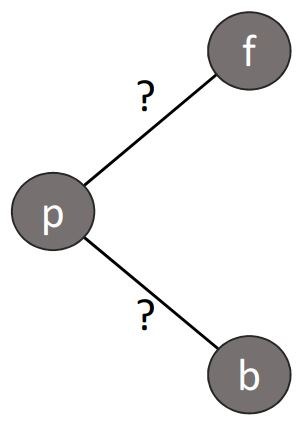
\includegraphics[height=3cm, width=2cm]{distance_between_f_b.jpg}
 	\caption{Foglie vicine con un generico genitore $p$.}
  	\label{fig:neighborsleaves}
\end{figure}
\newline
Come si può calcolare la distanza tra $f$ e $p$ ($d_{fp}$) e tra $b$ e $p$ ($d_{bp}$)? Le uniche informazioni a disposizione sono le distanze tra le quattro foglie presenti nella matrice e l'ipotesi che $f$ e $b$ siano vicine. Il passo successivo dell'algoritmo è mostrato di seguito.
\begin{figure}[h!]
\centering
	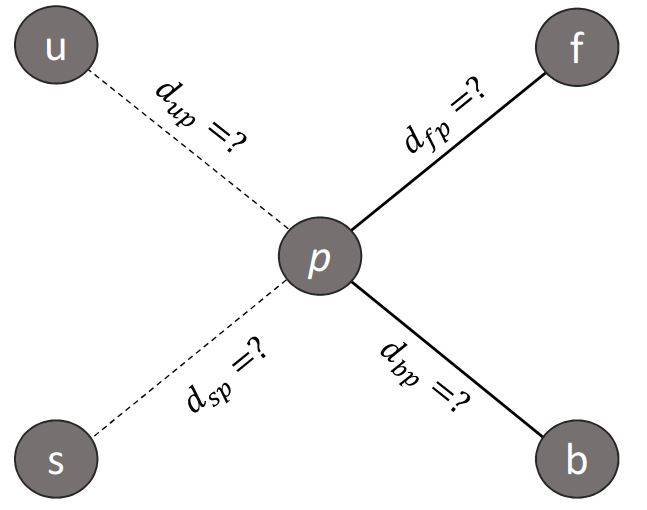
\includegraphics[height=9cm, width=7cm, keepaspectratio]{distance_between_f_b_part_2.jpg}
 	\caption{Le quattro foglie $u$, $s$, $f$ e $d$.}
  	\label{fig:neighborsleaves_2}
\end{figure}
\newline
Nella figura 8 sono state aggiunte le foglie $u$ ed $s$, ma il loro arco è tratteggiato in quanto ancora non è possibile sapere come sono collocate nell'albero.
\newline
In questo step viene scelta casualmente una foglia tra $u$ ed $s$ e viene sfruttato il valore della sua distanza rispetto a $p$ per poter calcolare $d_{fp}$ e $d_{bp}$ (in questo caso si sceglie $u$). Per far ciò è quindi necessario scrivere le distanze tra le foglie nel seguente modo:
\[d_{fu}=d_{fp}+d_{up}\]
\[d_{fb}=d_{fp}+d_{bp}\]
\[d_{bu}=d_{bp}+d_{up}\]
\[d_{up}=\frac{d_{fu}+d_{bu}-d_{fb}}2=
\frac{(d_{fp}+d_{up})+(d_{bp}+d_{up})-(d_{fp}+d_{bp})}2=\]
\[=\frac{d_{fp}+d_{up}+d_{bp}+d_{up}-d_{fp}-d_{bp}}2=
\frac{d_{up}+d_{up}}2=
\frac{2d_{up}}2=d_{up}
\]
Perché scrivere $d_{up}$ in quel modo? Perché non si conosce il peso dei nodi interni ma solo quello delle foglie grazie alla matrice di partenza, quindi vengono usate queste informazioni per calcolare la distanza tra $f$ e $p$ e tra $b$ e $p$ nell'albero $T$. Inoltre $D$ è additiva, questo significa che la distanza tra le foglie in $T$ è uguale alla distanza tra i rispettivi elementi nella matrice, pertanto $d_{fu}=D_{fu}$, $d_{fb}=D_{fb}$ e $d_{bu}=D_{bu}$\footnote{Si ricorda che $d_{fu}$ è la distanza tra il nodo $f$ ed il nodo $u$ nell'albero $T$, mentre $D_{fu}$ è l'elemento in posizione $f-u$ in $D$.}. Ma allora si può scrivere $d_{up}$ nel seguente modo:
\[d_{up}=\frac{d_{fu}+d_{bu}-d_{fb}}2=\frac{D_{fu}+D_{bu}-D_{fb}}2\]
A questo punto si è in grado di calcolare la distanza tra $f$ e $p$ e tra $b$ e $p$, ricavandola dalle uguaglianze trovate poc'anzi. Per prima cosa si calcola $d_{fp}$:
\[d_{fu}=d_{fp}+d_{up} \rightarrow d_{fp}=d_{fu}-d_{up}=D_{fu}-D_{up}=\]
\[=D_{fu}-\frac{D_{fu}+D_{bu}-D_{fb}}2=\frac{2D_{fu}-D_{fu}-D_{bu}+D_{fb}}2=\]
\[=\frac{D_{fu}+D_{fb}-D_{bu}}2=\frac{7+2-5}2=2\]
Quindi $d_{fp}=2$. In modo analogo si calcola $d_{bp}$:
\[d_{bu}=d_{bp}+d_{up} \rightarrow d_{bp}=d_{bu}-d_{up}=D_{bu}-D_{up}=\]
\[=D_{bu}-\frac{D_{fu}+D_{bu}-D_{fb}}2=\frac{2D_{bu}-D_{fu}-D_{bu}+D_{fb}}2=\]
\[\frac{D_{bu}+D_{fb}-D_{fu}}2=\frac{5+2-7}2=0\]
Quindi $d_{bp}=0$. Il risultato di questo passo dell'algoritmo è il seguente albero:
\begin{figure}[h!]
\centering
	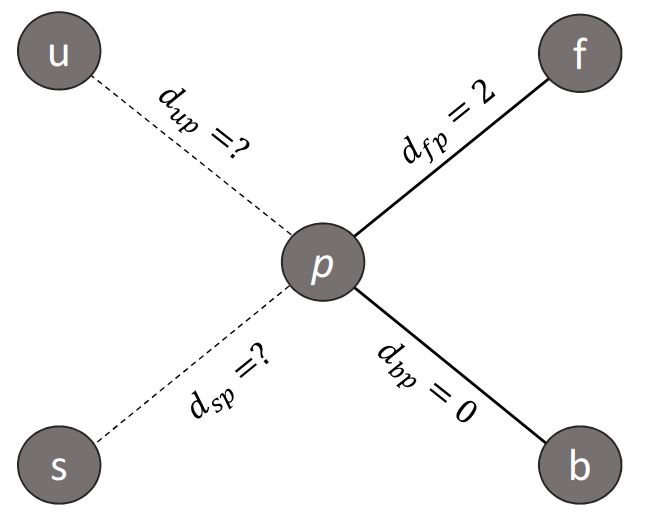
\includegraphics[height=9cm, width=7cm, keepaspectratio]{distance_between_f_b_part_3.jpg}
 	\caption{Albero con le distanze $d_{fp}$ e $d_{bp}$.}
  	\label{fig:neighborsleaves_3}
\end{figure}
\newline
Il prossimo step consiste nel trovare la distanza tra $u$ e $p$ e tra $s$ e $p$: dalla matrice D sappiamo che $D_{fu}=d_{fu}=7$ e dai calcoli precedenti che $d_{fp}=2$, quindi $d_{up}=d_{fu}-d_{fp}=7-2=5$. Stesso ragionamento anche per $d_{sp}$, ovvero $d_{sp}=d_{bs}-d_{bp}=4-0=4$.
\newline
L'albero corrispondente è:
\newpage
\begin{figure}[h!]
\centering
	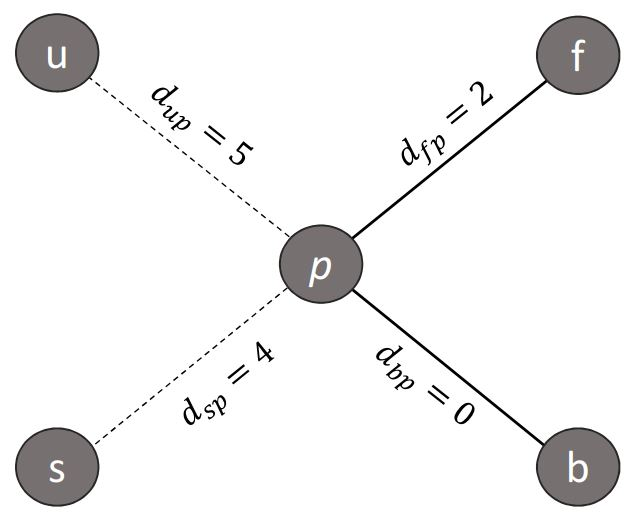
\includegraphics[height=9cm, width=7cm, keepaspectratio]{distance_between_f_b_part_4.jpg}
 	\caption{Albero con le distanze $d_{fp}$, $d_{bp}$, $d_{up}$ e $d_{sp}$.}
  	\label{fig:neighborsleaves_3}
\end{figure}
Adesso è necessario fare due modifiche alla matrice D, la prima consiste nel mettere una riga e colonna in più, definite $p$, che rappresentano le distanze appena trovate, ottenendo quindi la seguente matrice:
\[
D = \bordermatrix{\text{specie}&u&s&f&b&p\cr
                u& 0 & 3 & 7 & 5 & 5\cr
                s& 3 & 0 & 6 & 4 & 4\cr
                f& 7 & 6 & 0 & 2 & 2\cr
                b& 5 & 4 & 2 & 0 & 0\cr
                p&  5 & 4 & 2 & 0 & 0}
\]
la seconda invece consiste nel togliere le righe e colonne appartenenti a $f$ e $b$, in quanto i rispettivi nodi sono già aggiunti all'albero, pertanto non più utili. Quindi:
\[
D = \bordermatrix{\text{specie}&u&s&p\cr
                u& 0 & 3 & 5\cr
                s& 3 & 0 & 4\cr
                p&  5 & 4 & 0}
\]
Anche se adesso si conoscono le distanze di tutte le foglie con il genitore $p$, rimane comunque da capire se $u$ e $s$ abbiano altri genitori. Si ricorda, infatti, che i loro archi sono stati tratteggiati in quanto ancora non si conosce la loro collocazione nell'albero.
Per risolvere questo problema basta applicare ricorsivamente i passi precedenti, quindi si individua l'elemento più piccolo della matrice ($d_{su}$) e si suppone che $s$ e $u$ siano vicini e quindi che abbiano un genitore non noto $k$, come mostrato in figura 11.
\newpage
\begin{figure}[h!]
\centering
	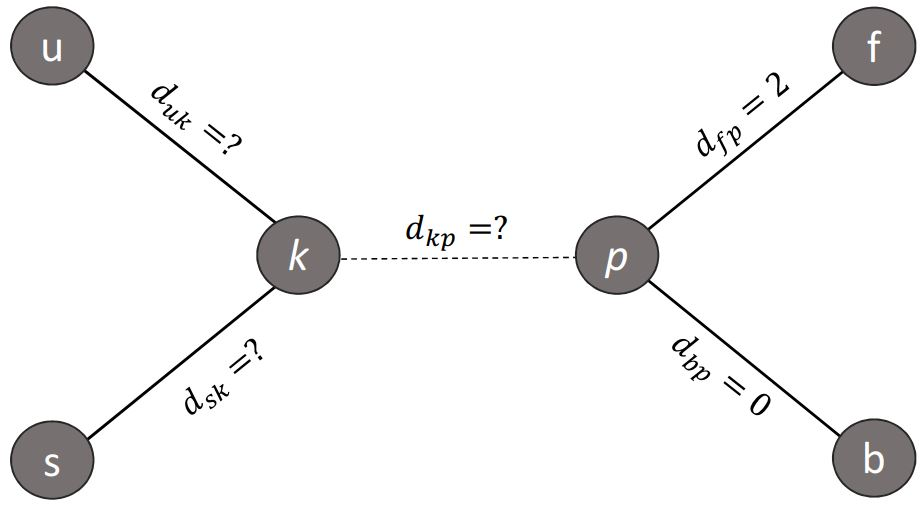
\includegraphics[height=13cm, width=11cm, keepaspectratio]{distance_between_s_u.jpg}
 	\caption{Albero con il nuovo genitore non noto $k$.}
  	\label{fig:neighborsleaves_3}
\end{figure}
Viene scelto il nodo $p$ e sfruttato il valore della sua distanza rispetto ad $u$ e $s$ per poter calcolare $d_{uk}$ e $d_{sk}$. Adattando le formule di pagina $31$ con i dati attuali, si ottiene:
\[d_{pk}=\frac{d_{up}+d_{sp}-d_{us}}2=
\frac{(d_{uk}+d_{pk})+(d_{sk}+d_{pk})-(d_{uk}+d_{sk})}2=\]
\[=\frac{2d_{pk}}2=d_{pk}
\]
Adesso si può calcolare $d_{uk}$:
\[d_{up}=d_{uk}+d_{pk} \rightarrow d_{uk}=D_{up}-D_{pk}=D_{up}-\frac{D_{up}+D_{sp}-D_{us}}2=\]
\[=\frac{D_{up}+D_{us}-D_{sp}}2=2\]

%-\frac{(D_{uk}+D_{pk})+(D_{sk}+D_{pk})-(D_{uk}+D_{sk})}2=\]
%\[=\frac{(D_{up}+D_{us}-D_{sp})}2=2
%\]
E $d_{sk}$:
\[d_{sp}=d_{sk}+d_{pk} \rightarrow d_{sk}=D_{sp}-D_{pk}=D_{sp}-\frac{D_{up}+D_{sp}-D_{us}}2=\]
\[=\frac{D_{sp}+D_{us}-D_{up}}2=1\]
Applicando le distanze trovate all'albero della figura 11, si ottiene:
\newpage
\begin{figure}[h!]
\centering
	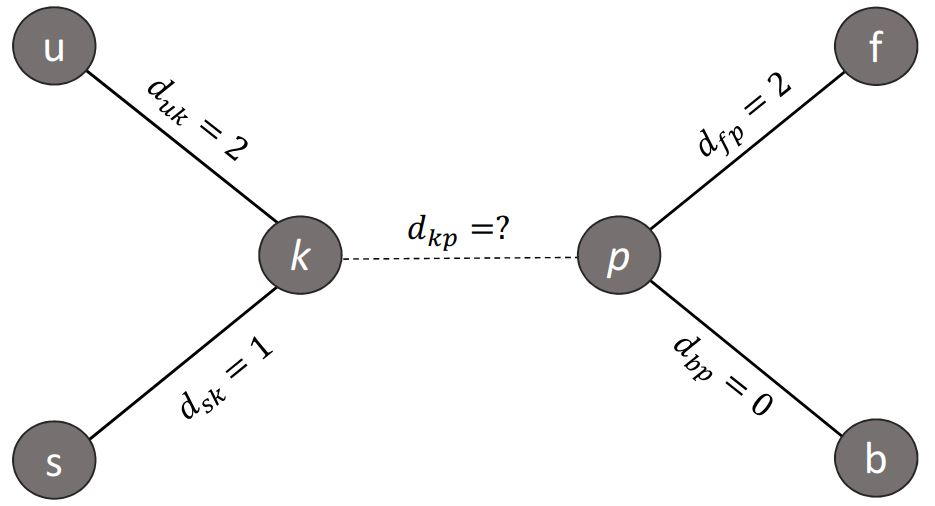
\includegraphics[height=13cm, width=11cm, keepaspectratio]{distance_between_s_u_part_2.jpg}
 	\caption{Albero con le distanze $d_{uk}$ e $d_{sk}$ calcolate.}
  	\label{fig:neighborsleaves_3}
\end{figure}
Dopo aver trovato ricorsivamente la distanza delle foglie dai propri genitori e di conseguenza aver aggiornato la matrice, rimane un ultimo passo da completare, ovvero calcolare la distanza tra $k$ e $p$: in precedenza si era calcolata la distanza tra $u$ e $p$ e tra $s$ e $p$, quindi basta sottrarre tali valori a quelli trovati adesso e troviamo $d_{kp}$.
\[d_{kp}=d_{sp}-d_{sk}=4-1=d_{up}-d_{uk}=5-2=3\]
L'albero finale che si ottiene è il seguente:
\begin{figure}[h!]
\centering
	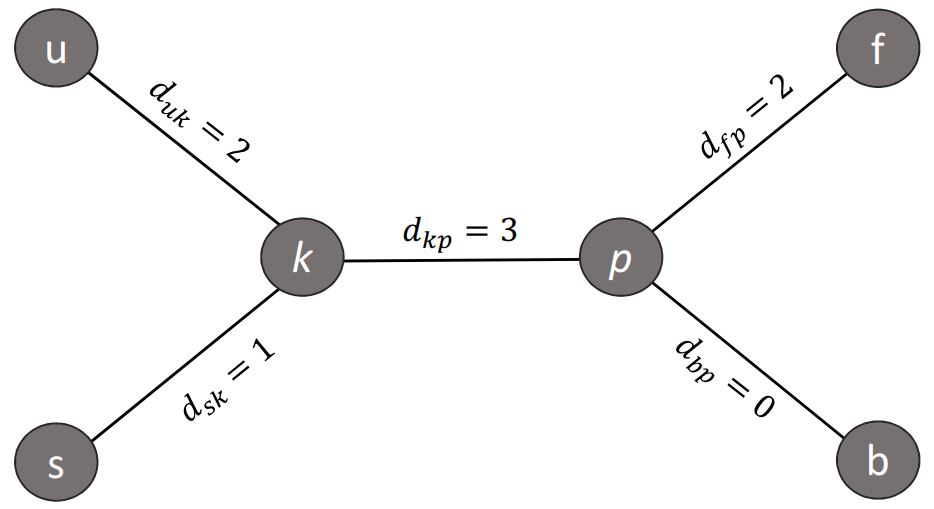
\includegraphics[height=13cm, width=11cm, keepaspectratio]{distance_between_s_u_part_4.jpg}
 	\caption{Albero evolutivo semplice con tutte le distanze calcolate.}
  	\label{fig:neighborsleaves_4}
\end{figure}
\newline
L'algoritmo è terminato. Tuttavia vi è una criticità che viene mostrata nella sezione successiva.

\subsection{Complessità temporale}
Per calcolare la complessità nel tempo dell'algoritmo possiamo suddividerlo in tre step, di seguito elencati.
\begin{enumerate}
	\item \textit{Step 1}: Trovare il minimo in una matrice di dimensione $n \times n$.
	\newline
	Si suppone l'utilizzo di un algoritmo di ricerca lineare, la cui complessità nel caso pessimo, dato in input un vettore di lunghezza $n$, è pari a $O(n)$. Poiché questa operazione deve essere effettuata per tutte le $n$ righe, otteniamo che:
	\[T(step 1)=O(n) \times O(n) = O(n^2)\]
	\item \textit{Step 2}: Trovare il genitore per ogni coppia di foglie e calcolare la distanza di tutte le $n$ foglie  rispetto al genitore stesso.
	\newline
	Questa operazione deve essere fatta $n$ volte, quindi $O(n)$. In seguito dovrà essere aggiornata la matrice; per semplicità si suppone che il costo rimanga invariato, quindi $O(1)$.
	\[T(step 2)=O(n)+O(1) \simeq O(n)\]
	\item \textit{Step 3}: Calcolare le distanze tra i genitori trovati nello step precedente.
	\newline
	Poiché per ogni coppia di foglie esiste un genitore, allora il costo sarà:
	\[T(step 3)=O(n/2)\]
\end{enumerate}
Adesso è sufficiente sommare le tre complessità e si trova quella totale dell'algoritmo:
\[T(totale)=T(step 1)+T(step 2)+T(step 3)=\]
\[=O(n^2)+O(n)+O(n/2) \simeq O(n^2) \]

\newpage

\section{Albero Additivo}
L'algoritmo mostrato nella sezione precedente presenta una criticità, infatti riesce a risolvere il problema degli \textit{alberi basati sulla distanza} solamente se l'elemento più piccolo della matrice D corrisponde a due foglie \textit{vicine} nell'albero T. Ma questo non è necessariamente vero, infatti ci sono matrici delle distanze che, seppur additive (e quindi $ \forall i,j\in V,D_{ij}=d_{ij}(T)$), non possiedono come elemento più piccolo una coppia di foglie con lo stesso genitore. Pertanto si deve approcciare il problema in modo diverso: invece di cercare le foglie vicine in un albero (come visto nella sezione precedente), l'idea di base dell'algoritmo è quella di costruirlo aggiungendole una alla volta. Per far ciò è necessario conoscere il peso degli archi che collegano le foglie ai rispettivi genitori. Questi prendono il nome di \textit{arti}. Tutti gli altri sono definiti \textit{archi interni} \cite{dataMiningInBioinformatics}. Tale operazione andrà effettuata in termini di matrice delle distanze D, dato che non si conosce l'albero T fino a che l'algoritmo non è terminato.
\newline
Il primo problema che si pone è quello di calcolare il peso degli arti: data una foglia $j$, si denota con \textit{limbweight(j)} il peso dell'arco che collega $j$ al suo genitore \cite{introductionbioinfalg}.
\newline
\newline
\textbf{Teorema del peso degli arti:}
\newline
\textit{Data una matrice delle distanze additiva $D$ ed una foglia $j$, \textit{limbweight(j)} è uguale al valore minimo di $\frac{D_{j,i}+D_{j,k}-D_{i,k}}{2}$ tra tutte le foglie $i$ e $k$\footnote{Si omette la dimostrazione, che è consultabile al capitolo 7 del libro \textit{Bioinformatics Algorithms, An Active Learning Approach, Vol II} di Compeau P., Pevzner P.} \cite{bioinfalganactivelearningapproachparttwo}} .
\newline
\newline
A titolo esemplificativo si riporta l'applicazione del teorema alla seguente matrice\footnote{Per brevità si definisce f=foca, b=balena, u=umano, s=scimpanzé. Inoltre si ricorda che questi rappresentano le foglie nel rispettivo albero evolutivo $T$.}:
\[
D = \bordermatrix{\text{specie}&u&s&f&b\cr
                u& 0 & 3 & 7 & 5\cr
                s& 3 & 0 & 6 & 4\cr
                f& 7 & 6 & 0 & 2\cr
                b& 5 & 4 & 2 & 0}
\]
Supponendo di non conoscere quali sono le foglie vicine, si vuole calcolare il peso dell'arto di $f$, quindi:
\[limbweight(f)=\frac{D_{f,i}+D_{f,k}-D_{i,k}}{2}\]
Al posto $i$ e $k$ si sostituiscono di volta in volta i valori delle foglie (escluso $f$), ovvero:
\begin{itemize}
	\item $i=u$ e $k=s$:
	\[limbweight_{us}(f)=\frac{D_{f,u}+D_{f,s}-D_{u,s}}{2}=\frac{7+6-3}{2}=\frac{10}{2}=5\]
	\item $i=u$ e $k=b$:
	\[limbweight_{ub}(f)=\frac{D_{f,u}+D_{f,b}-D_{u,b}}{2}=\frac{7+2-5}{2}=\frac{4}{2}=2\]
	\item $i=s$ e $k=b$:
	\[limbweight_{sb}(f)=\frac{D_{f,s}+D_{f,b}-D_{s,b}}{2}=\frac{6+2-4}{2}=\frac{4}{2}=2\]
\end{itemize}
Si può concludere dicendo che \textit{limbweight(f)}=$2$.
\newline
Tali operazioni hanno una complessità di $O(n^2)$, in quanto ogni $i-esimo$  elemento della matrice $n \times n$ viene confrontato con tutti gli altri $k$ elementi (con $k>i$), che sono $n-3$ (escluso $f$, $i$  e sé stesso). Questa operazione viene eseguita tante volte quante sono le foglie da analizzare, ovvero $n$, quindi $\rightarrow T(limbweight(f))=O(n-3)\times O(n)\simeq O(n^2)$.
\newline
Ora che si è in grado di calcolare il peso degli arti si può illustrare l'algoritmo che risolve la criticità spiegata ad inizio della sezione.
\newline
Sia $D$ una matrice delle distanze additiva di dimensione $n\times n$, tale che il suo elemento più piccolo \textbf{non} corrisponda a due foglie \textit{vicine} nel rispettivo albero $T$\footnote{Per capire se l'elemento più piccolo di una matrice corrisponda ad una coppia di foglie vicine nel rispettivo albero è necessario eseguire l'algoritmo della sezione precedente (sezione $4.3$) usando la matrice $D$ in input. In tal caso il peso di alcuni archi sarebbe risultato negativo e quindi non sarebbe possibile costruire $T$. }, ovvero:
\[
D = \bordermatrix{\text{specie}&f&b&u&s\cr
                f& 0 & 13 & 21 & 22\cr
                b& 13 & 0 & 12 & 13\cr
                u& 21 & 12 & 0 & 13\cr
                s& 22 & 13 & 13 & 0}
\]
\newpage
L'albero che si intende ottenere è il seguente:
\begin{figure}[h!]
\centering
	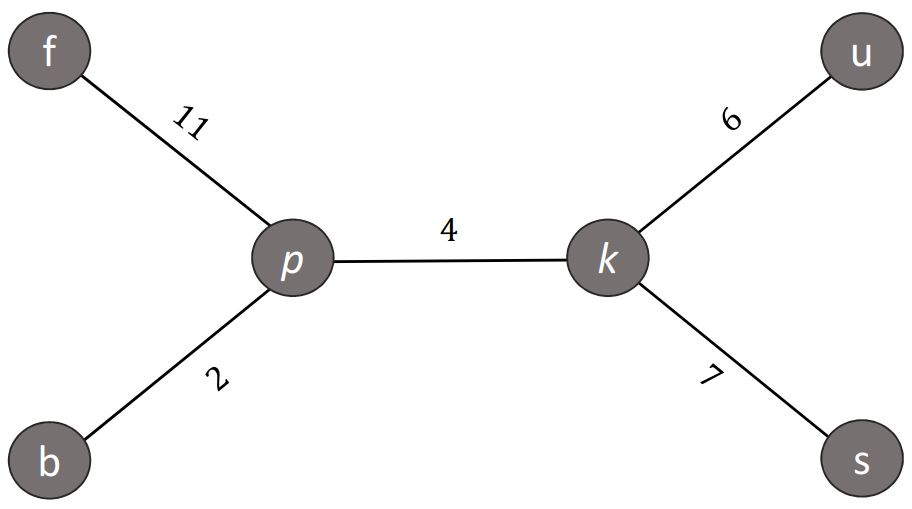
\includegraphics[height=12cm, width=10cm, keepaspectratio]{additive_tree_1.jpg}
 	\caption{Albero T ottenuto dalla matrice D.}
  	\label{fig:additivePhylogeny_1}
\end{figure}
\newline
Per prima cosa si sceglie casualmente dalla matrice una foglia $b$ e si calcola \textit{limbweight(b)}:
\[limbweight(b)=\frac{D_{b,i}+D_{b,k}-D_{i,k}}{2}\]
\begin{itemize}
	\item $i=f$ e $k=u$:
	\[limbweight_{fu}(b)=\frac{D_{b,f}+D_{b,u}-D_{f,u}}{2}=\frac{13+12-21}{2}=\frac{4}{2}=2\]
	\item $i=f$ e $k=s$:
	\[limbweight_{fs}(b)=\frac{D_{b,f}+D_{b,s}-D_{f,s}}{2}=\frac{13+13-22}{2}=\frac{4}{2}=2\]
	\item $i=u$ e $k=s$:
	\[limbweight_{us}(b)=\frac{D_{b,u}+D_{b,s}-D_{u,s}}{2}=\frac{12+13-13}{2}=\frac{12}{2}=6\]
\end{itemize}
Quindi $limbweight(b)=2$.
\newline
Adesso è necessario aggiornare la matrice, sottraendo $limbweight(b)$ a tutti gli elementi lungo la riga e la colonna $b$ (escluso lo zero sulla diagonale). Quindi si ottiene una nuova matrice $D^{spoglia_{b}}$ che verrà utilizzata successivamente per costruire l'albero.
\[
D^{spoglia_{b}}= \bordermatrix{\text{specie}&f&b&u&s\cr
                f& 0 & {\color{Blue} 11} & 21 & 22\cr
                b& {\color{Blue} 11} & 0 & {\color{Blue} 10} & {\color{Blue} 11}\cr
                u& 21 & {\color{Blue} 10} & 0 & 13\cr
                s& 22 & {\color{Blue} 11} & 13 & 0}
\]
Poiché la riga e la colonna $b$ non forniscono informazioni aggiuntive, sarebbe inutile tenerle, pertanto si eliminano dalla matrice $D^{spoglia_{b}}$. Il risultato è il seguente:
\[
D^{tagliata_{b}}= \bordermatrix{\text{specie}&f&u&s\cr
                f& 0 & 21 & 22\cr
                u& 21 & 0 & 13\cr
                s& 22 & 13 & 0}
\]
Adesso si può ottenere l'albero evolutivo $T$ eseguendo ricorsivamente i seguenti step:
\begin{enumerate}
	\item Scegliere casualmente una foglia $j$, calcolare $limbweight(j)$, costruire $D^{spoglia_{j}}$ e  $D^{tagliata_{j}}$. Ripetere queste operazioni fino a che non si ottiene una matrice $D^{tagliata}$ di dimensioni $2 \times 2$.
	\item Costruire un albero $T^{tagliato}$ a partire da $D^{tagliata}$ trovata nello step precedente. All'inizio sarà composto solamente da una coppia di foglie ed un arco che le collega.
	\item Identificare il punto di $T^{tagliato}$ in cui la foglia $j$ deve essere inserita. Questo passo dell'algoritmo verrà spiegato successivamente.
	\item Aggiungere la foglia $j$ ed aggiornare il peso degli archi in $T^{tagliato}$. La ripetizione di questo punto e di quello precedente permettono la costruzione dell'albero di volta in volta fino al suo completamento.
\end{enumerate}
Si applicano i passaggi sopraelencati alla matrice $D^{tagliata_{b}}$, quindi si sceglie la foglia $s$ e si calcola \textit{limbweight(s)}:
\[limbweight(s)=\frac{D_{s,i}+D_{s,k}-D_{i,k}}{2}\]
\begin{itemize}
	\item $i=f$ e $k=u$:
	\[limbweight(s)=\frac{D_{s,f}+D_{s,u}-D_{f,u}}{2}=\frac{22+13-21}{2}=\frac{14}{2}=7\]
\end{itemize}
Si sottrae $limbweight(s)=7$ a tutti gli elementi lungo la riga e la colonna $s$ in $D^{tagliata_{b}}$, ottenendo così:
\[
D^{spoglia_{s}}= \bordermatrix{\text{specie}&f&u&s\cr
                f& 0 & 21 & {\color{Blue} 15}\cr
                u& 21 & 0 & {\color{Blue} 6}\cr
                s& {\color{Blue} 15} & {\color{Blue} 6} & 0}
\]
A questo punto si elimina la foglia $s$ da $D^{spoglia_{s}}$:
\[
D^{tagliata_{s}}= \bordermatrix{\text{specie}&f&u\cr
                f& 0 & 21\cr
                u& 21 & 0}
\]
Il risultato è una matrice $2 \times 2$, quindi si può cominciare a costruire l'albero:
\begin{figure}[h!]
\centering
	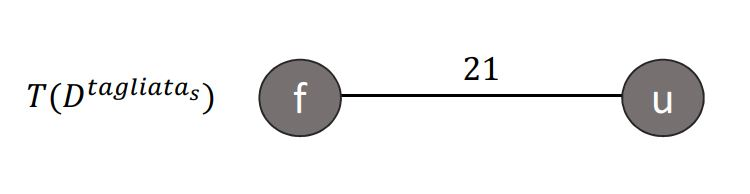
\includegraphics[height=9cm, width=7cm, keepaspectratio]{additive_tree_2.jpg}
 	\caption{Albero ottenuto dalla matrice $D^{tagliata_{s}}$.}
  	\label{fig:additivePhylogeny_2}
\end{figure}
\newline
Lo step successivo è quello di individuare il punto in $T(D^{tagliata_{s}})$ in cui $s$ deve essere inserito. Per fare ciò si consideri la matrice $D^{spoglia_{s}}$. Dal \textit{teorema del peso degli arti} si ha che:
\[limbweight(s)=\frac{D^{spoglia_{s}}_{f,s}+D^{spoglia_{s}}_{s,u}-D^{spoglia_{s}}_{f,u}}{2}\]
Ma poiché $D^{spoglia_{s}}$ è una matrice ottenuta da $D^{tagliata_{b}}$ togliendo il peso dell'arto di $s$, allora $limbweight(s)=0$. Quindi:
\[
0=\frac{D^{spoglia_{s}}_{f,s}+D^{spoglia_{s}}_{s,u}-D^{spoglia_{s}}_{f,u}}{2} \rightarrow D^{spoglia_{s}}_{f,u}=D^{spoglia_{s}}_{f,s}+D^{spoglia_{s}}_{s,u}
\]
Questo significa che il punto di attacco di $s$  è lungo l'arco che collega $f$ con $u$\footnote{Il punto di attacco può essere anche su un vertice già esistente, in tal caso si connette $s$ a tale vertice.}, quindi si crea un nodo interno $k$ che rappresenta il genitore di $s$, si aggiunge la foglia $s$ connettendola proprio a $k$ tramite un arto di peso pari a limbweight(s) = 7 e si aggiorna il peso degli altri archi, quindi:
\newpage
\begin{figure}[h!]
\centering
	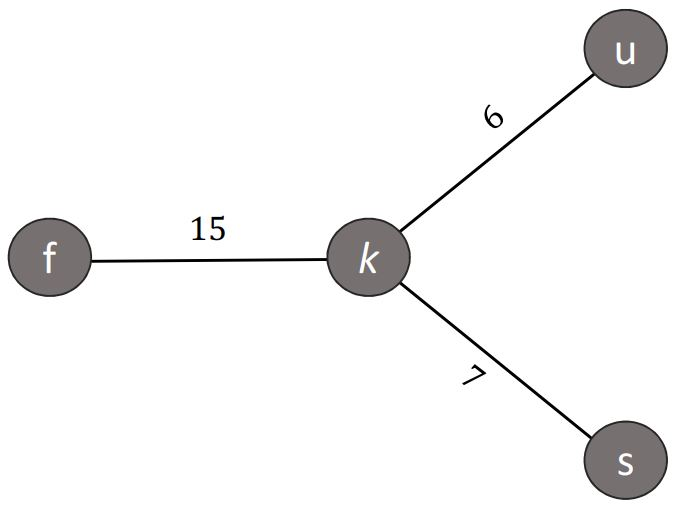
\includegraphics[height=8cm, width=6cm, keepaspectratio]{additive_tree_3.jpg}
 	\caption{Albero con la nuova foglia $s$.}
  	\label{fig:additivePhylogeny_3}
\end{figure}
$d_{sk}=7$ è il peso dell'arto di $s$ che è già stato calcolato in precedenza; $d_{uk}=D^{spoglia_{s}}_{s,u}=6$ è ottenuto sottraendo $limbweight(s)=7$ a \newline $D^{tagliata_{b}}_{s,u}=13$; $d_{fk}=15$ è dato da $D^{spoglia_{s}}_{f,u}-d_{uk}=21-6=15$.
\newline
Si ripetono gli ultimi step dell'algoritmo fino a che non si ottiene l'albero $T$, quindi si individua il punto in figura 16 in cui $b$ deve essere inserito.
\[
limbweight(b)=\frac{D^{spoglia_{b}}_{f,b}+D^{spoglia_{b}}_{b,u}-D^{spoglia_{b}}_{f,u}}{2} \rightarrow\]
\[ \rightarrow limbweight(b)=0,\: quindi\rightarrow 0=\frac{D^{spoglia_{b}}_{f,b}+D^{spoglia_{b}}_{b,u}-D^{spoglia_{b}}_{f,u}}{2}\rightarrow\]
\[\rightarrow D^{spoglia_{b}}_{f,u}=D^{spoglia_{b}}_{f,b}+D^{spoglia_{b}}_{b,u}
\]
Analogamente al passaggio effettuato poc'anzi, si nota che il punto di attacco di $b$ è lungo l'arco che collega $f$ con $u$, quindi si crea un nodo interno $p$ che rappresenta il genitore di $b$,
si aggiunge la foglia $b$ connettendola a $p$ tramite un arto di peso pari a
$limbweight(b)=2$ e si aggiorna il peso degli altri archi.
\newpage
L'albero evolutivo è il seguente:
\begin{figure}[h!]
\centering
	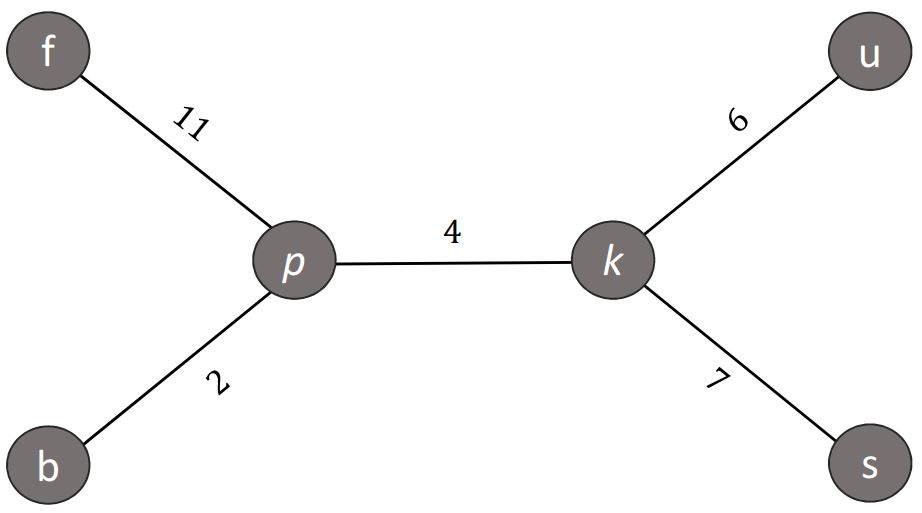
\includegraphics[height=13cm, width=11cm, keepaspectratio]{additive_tree_4.jpg}
 	\caption{Albero $T$ ottenuto da $D$.}
  	\label{fig:additivePhylogeny_4}
\end{figure}
\newline
$d_{bp}=2$ è il peso dell'arto di $b$ che è già stato calcolato in precedenza; $d_{fp}=D^{spoglia_{b}}_{f,b}=11$ è ottenuto sottraendo $limbweight(b)=2$ a $D_{f,b}=13$; $d_{pk}=4$ è dato dalla sottrazione tra $d_{fk}$ (figura 16) e $d_{fp}=D^{spoglia_{b}}_{f,b}$, quindi $d_{fk}-d_{fp}=15-11=4$.
\newline
Poiché è stato costruito l'albero nella sua interezza, l'algoritmo è terminato. Tuttavia anche in questo caso vi è una criticità, in quanto riesce a costruire $T$ \textit{se e solo se} la matrice $D$ è additiva, ed in molti casi non è così.
\newline
Nella sezione successiva viene mostrato un algoritmo che risolve tale criticità.

\newpage
\subsection{Complessità temporale}
Di seguito viene riportato l'algoritmo scritto in pseudocodice. I parametri sono D ed n, che sono rispettivamente la matrice delle distanze adattiva di dimensione $n \times n$ e la foglia $n$.

\begin{framed}\noindent
  \textbf{AlberoAdditivo($D$, $n$)}\\
  \textbf{se} $n=2$\\
  \indent \textbf{Restituisci} l'albero costituito da un arco che collega le due foglie\\
  \textbf{altrimenti} esegui le seguenti operazioni: \\
  pesoArto $\leftarrow$ \textbf{limbweight}(n)\\
  \textbf{per} $j \leftarrow 1$ \textbf{fino a} $n-1$\\
  \indent $D_{jn} \leftarrow D_{jn} - pesoArto$\\
  \indent $D_{nj} \leftarrow D_{jn}$\\
  ($i$,$n$,$k$) $\leftarrow$ tre foglie tale che $D_{ik}=D_{in}+D_{nk}$\\
  $x \leftarrow D_{in}$\\
  \textbf{rimuovi} la riga e la colonna $n$ dalla matrice D \\
  $T \leftarrow $\textbf{AlberoAdditivo($D$, $n-1$)}\\
  $v \leftarrow $ il genitore di $n$ che è distante $x$ rispetto ad $i$ in $T$, dove $i$ è la foglia vicina di $n$\\
  %\footnote{In altre parole è il nodo interno che viene inserito prima di poter 	  mettere la foglia (nella figura 17 sono $k$ e $p$.)} \\
  \textbf{aggiungi} la foglia $n$ a $T$ creando un arto tra $v$ ed $n$ il cui peso è \textit{pesoArto}
\end{framed}
Ogni volta che l'algoritmo richiama sé stesso, vengono eseguite le seguenti operazioni:
\begin{enumerate}
	\item calcola il peso dell'arto dell'$n-esima$ foglia $\rightarrow T(step 1) \simeq O(n^2)$\footnote{Si ricorda che la complessità di \textit{limbweight} è $O(n^2)$.};
	\item aggiorna i valori della matrice $\rightarrow T(step 2) \simeq O(n-1)$;
	\item individua il punto in cui va inserita l'$n-esima$ foglia ed elimina la riga e la colonna $n$. Poiché questo step esegue sempre lo stesso numero di operazioni, possiamo considerare la sua complessità come costante $\rightarrow  T(step 3) \simeq O(1)$.  
\end{enumerate} 
Quindi:
\[T(AlberoAdditivo)=T(step 1)+T(step 2)+T(step 3)=\]
\[=O(n^2)+O(n-1)+O(1) \simeq O(n^2)\]
Ma \textit{AlberoAdditivo} viene eseguito $n$ volte, ovvero fino a che non si costruisce un albero $T$ con $n$ foglie, pertanto la complessità totale dell'algoritmo è:
\[T(totale)=T(AlberoAdditivo) \times O(n)=O(n^2) \times O(n)= O(n^3)\]

\newpage

\section{Algoritmo Neighbor-Joining}
Gli algoritmi precedentemente elencati mostrano delle criticità, in quanto il primo riesce a costruire l'albero $T$ solo se la matrice additiva $D$ ha come elemento più piccolo una coppia di foglie vicine in $T$, mentre il secondo, anche se risolve questo problema, non riesce a costruirlo se $D$ non è additiva.
\newline
\`E necessario fare una precisazione: non c'è modo che un albero si \textit{adatti} ad una matrice \textit{non additiva}, proprio per definizione della stessa, tuttavia è possibile costruire un albero che approssimi al meglio la distanza tra le foglie della matrice attraverso uno degli algoritmi più importanti della bioinformatica, il \textbf{Neighbor-Joining}. Nel caso in cui la matrice sia \textit{additiva}, allora il \textbf{NJ} costruisce un albero che si adatta ad essa.
\newline
Si prenda in considerazione la seguente matrice \textit{non additiva}\footnote{Per brevità si definisce u=umano, s=scimpanzé, f=foca, b=balena.}:
\[
D = \bordermatrix{\text{specie}&f&b&u&s\cr
                f& 0 & 3 & 4 & 3\cr
                b& 3 & 0 & 4 & 5\cr
                u& 4 & 4 & 0 & 2\cr
                s& 3 & 5 & 2 & 0}
\]
L'obiettivo è quello di costruire un albero $T$ che approssimi al meglio le distanze tra le foglie in $D$.
\newline
Il \textit{primo} passo dell'algoritmo Neighbor-Joining consiste nel trovare $D^\star$. Dato in input $D$ si definisce $D^\star$ la seguente matrice \cite{neighborjoinrevealed}:
\[\forall \,f,b\in D,\: \, D^\star(f,b)=(n-2)\cdot D(f,b)-\sum_{k=1}^{n}D(f,k)-\sum_{k=1}^{n}D(b,k)\]
dove $totalDistance(D_f)=\sum_{k=1}^{n}D(f,k)$ e $totalDistance(D_b)=$\newline$=\sum_{k=1}^{n}D(b,k)$.
La sua caratteristica principale è che qualunque sia la matrice delle distanze in input, l'elemento più piccolo della relativa matrice $D^\star$ corrisponde ad una coppia di foglie \textit{vicine} nell'albero $T$. 
\newline
Quindi prima si trovano i valori di $totalDistance$ per ogni riga di $D$:
\[
D = \bordermatrix{\text{specie}&f&b&u&s\cr
                f& 0 & 3 & 4 & 3\cr
                b& 3 & 0 & 4 & 5\cr
                u& 4 & 4 & 0 & 2\cr
                s& 3 & 5 & 2 & 0}\;\;\;\;
\begin{matrix}
totalDistance(D_f)=10\\ 
totalDistance(D_b)=12\\ 
totalDistance(D_u)=10\\
totalDistance(D_s)=10
\end{matrix}
\]
Infine si calcolano i valori per creare $D^\star$:
\begin{itemize}
	\item $D^\star(f,b)=(4-2)\cdot D(f,b)-totalDistance(D_f)-totalDistance(D_b)=\\=2\cdot3-10-12=-16$
	\item $D^\star(f,u)=(4-2)\cdot D(f,u)-totalDistance(D_f)-totalDistance(D_u)=\\=2\cdot4-10-10=-12$
	\item $D^\star(f,s)=(4-2)\cdot D(f,s)-totalDistance(D_f)-totalDistance(D_s)=\\=2\cdot3-10-10=-14$	
	\item $D^\star(b,u)=(4-2)\cdot D(b,u)-totalDistance(D_b)-totalDistance(D_u)=\\=2\cdot4-12-10=-14$	
	\item $D^\star(b,s)=(4-2)\cdot D(b,s)-totalDistance(D_b)-totalDistance(D_s)=\\=2\cdot5-12-10=-12$
	\item $D^\star(u,s)=(4-2)\cdot D(u,s)-totalDistance(D_u)-totalDistance(D_s)=\\=2\cdot2-10-10=-16$
\end{itemize}
Quindi la matrice è:
\[D^\star = \bordermatrix{\text{specie}&f&b&u&s\cr
                f& 0 & -16 & -12 & -14\cr
                b& -16 & 0 & -14 & -12\cr
                u& -12 & -14 & 0 & -16\cr
                s& -14 & -12 & -16 & 0}
\]
A questo punto si può passare al \textit{secondo} step: si cerca l'elemento minimo in $D^\star$, ovvero $D^\star_{fb}$\footnote{Anche $D^\star_{us}$ è l'elemento più piccolo, tuttavia non se ne può scegliere più di uno alla volta.}, le cui foglie $f$ e $b$ sono \textit{vicine} in $T$.
\newline
Nel \textit{terzo} invece si calcola il \textit{delta} tra $totalDistance(D_f)$ e $totalDistance(D_b)$, quindi:
\[\Delta_{fb}=\frac{totalDistance(D_f)-totalDistance(D_b)}{n-2}=\frac{10-12}{4-2}=-1\]
Questo valore ci serve per il \textit{quarto} step, ovvero trovare il peso dell'arto di $f$ e di $b$:
\[limbweight(f)=\frac{D_{fb}+\Delta_{fb}}{2}=\frac{3+(-1)}{2}=1\]
\[limbweight(b)=\frac{D_{fb}-\Delta_{fb}}{2}=\frac{3-(-1)}{2}=2\]
Poiché si sono ottenute tutte le informazioni necessarie per poter inserire $f$ e $b$ nell'albero, si esegue lo step \textit{cinque}: si inserisce il loro genitore non noto in $D$, ovvero una riga e colonna $p$ tale che $\forall u\in D\setminus \, \{f,b\}, \; D_{up}=\frac{D_{fu}+D_{bu}-D_{fb}}{2}$ e si rimuovono le righe e le colonne di $f$ e di $b$. Quindi:
\[D_{up}=\frac{D_{fu}+D_{bu}-D_{fb}}{2}=\frac{4+4-3}{2}=\frac{5}{2}=2,5\]
\[D_{sp}=\frac{D_{fs}+D_{bs}-D_{fb}}{2}=\frac{3+5-3}{2}=\frac{5}{2}=2,5\]
Si può notare che la distanza di entrambe le foglie dal genitore sia la stessa. La matrice risultante è:
\[
D = \bordermatrix{\text{specie}&p&u&s\cr
                p& 0 & 2,5 & 2,5\cr
                u& 2,5 & 0 & 2\cr
                s& 2,5 & 2 & 0}
\]
I cinque passi sopraelencati devono essere eseguiti fino a che non si ottiene una matrice $2 \times 2$, quindi, \textit{step uno} $\rightarrow$ si calcolano $totalDistance(D_p)$,\newline $totalDistance(D_u)$, $totalDistance(D_s)$ e si costruisce $D^\star$:
\[
\begin{matrix}
totalDistance(D_p)=5\\ 
totalDistance(D_u)=4,5\\ 
totalDistance(D_s)=4,5
\end{matrix}\;\;\;\;
D^\star = \bordermatrix{\text{specie}&p&u&s\cr
                p& 0 & -7 & -7\cr
                u& -7 & 0 & -7\cr
                s& -7 & -7 & 0}
\]
\textit{Step due e tre} $\rightarrow$ si sceglie un elemento minimo in $D^\star$ (ovvero $D^\star_{us}$) e si calcola $Delta_{us}$, quindi:
\[\Delta_{us}=\frac{totalDistance(D_u)-totalDistance(D_s)}{n-2}=\frac{4,5-4,5}{3-2}=0\]
\textit{Step quattro} $\rightarrow$ si trovano i pesi degli arti di $u$ e di $s$. Poiché il \textit{delta} è uguale a zero, $limbweight(u)$ e $limbweight(s)$ hanno lo stesso valore:
\[limbweight(u)=\frac{D_{us}+\Delta_{us}}{2}=\frac{2+0}{2}=1\]
\[limbweight(s)=\frac{D_{us}-\Delta_{us}}{2}=\frac{2-0}{2}=1\]
\textit{Step cinque} $\rightarrow$ si inserisce il genitore non noto $k$ in $D$ aggiornando i valori della matrice e si eliminano $u$ ed $s$. Quindi:
\[D_{pk}=\frac{D_{up}+D_{sp}-D_{us}}{2}=\frac{2,5+2,5-2}{2}=\frac{3}{2}=1,5\]
La matrice che si ottiene è la seguente:
\[
D = \bordermatrix{\text{specie}&p&k\cr
                p& 0 & 1,5\cr
                k& 1,5 & 0}
\]
Poiché $D$ è di dimensione $2 \times 2$, si passa alla costruzione dell'albero.  Dalla matrice si ricava che $p$ e $k$ sono dei nodi interni legati tramite un arco di peso $1,5$, quindi:
\begin{figure}[h!]
\centering
	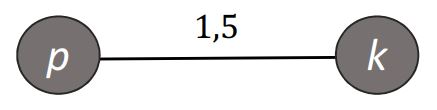
\includegraphics[height=7cm, width=5cm, keepaspectratio]{neighbor_joining_1.jpg}
 	\caption{Albero iniziale $T$.}
  	\label{fig:neighbor_joining_1}
\end{figure}
\newline
Come già specificato nei passi precedenti, $p$ e $k$ sono i genitori rispettivamente di $f$, $b$ e $u$, $s$, i cui pesi degli arti sono già stati calcolati, pertanto si può costruire direttamente l'albero evolutivo finale $T$:
\begin{figure}[h!]
\centering
	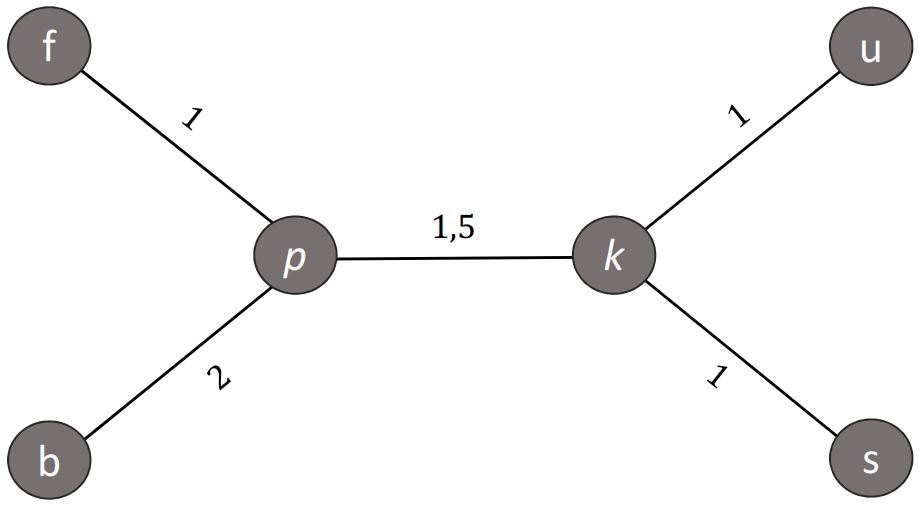
\includegraphics[height=13cm, width=11cm, keepaspectratio]{neighbor_joining_2.jpg}
 	\caption{Albero $T$ ottenuto dalla matrice delle distanze non additiva $D$.}
  	\label{fig:neighbor_joining_2}
\end{figure}
\newline
Si può notare che l'albero ottenuto non si adatta completamente alla matrice $D$ in quanto, come detto all'inizio della sezione, non è possibile ottenerlo a causa della non additività di $D$. \`E comunque possibile misurare quanto $T$ si adatti alla matrice attraverso la seguente formula \cite{understandingBioinf}:
\[Discrepancy(D(T),D)=\sum_{i=1}^{j-1}\sum_{j=i+1}^{n}(D_{ij}(T)-D_{ij})^2\]
Dove $D(T)$ è la matrice ottenuta da $T$, ovvero:
\[
D(T) = \bordermatrix{\text{specie}&f&b&u&s\cr
                f& 0 & 3 & 3,5 & 3,5\cr
                b& 3 & 0 & 4,5 & 4,5\cr
                u& 3,5 & 4,5 & 0 & 2\cr
                s& 3,5 & 4,5 & 2 & 0}
\]
Pertanto $Discrepancy(D(T),D)$ è:
\[Discrepancy(D(T),D)=(D_{1,2}(T)-D_{1,2})^2+(D_{1,3}(T)-D_{1,3})^2+\]
\[+(D_{1,4}(T)-D_{1,4})^2+(D_{2,3}(T)-D_{2,3})^2+(D_{2,4}(T)-D_{2,4})^2=\]
\[=0+(3,5-4)^2+(3,5-3)^2+(4,5-4)^2+(4,5-5)^2+0=1\]
Il risultato mostra che non c'è una grande discrepanza tra $D(T)$ e $D$, pertanto $T$ approssima al meglio la matrice in input.


\newpage
\subsection{Complessità temporale}
Si riporta l'algoritmo Neighbor-Joining in pseudocodice, dove $D$ è la matrice delle distanze additiva o non e $n$ è rispettivo il numero di righe e di colonne:
\begin{framed}\noindent
  \textbf{NeighborJoining($D$, $n$)}\\
  \textbf{se} $n=2$\\
  \indent \textbf{Restituisci} l'albero $T$ ottenuto da D costituito da un arco che collega le due foglie\\
  \textbf{altrimenti} esegui le seguenti operazioni: \\
  $D^\star \leftarrow $ matrice ottenuta da $D$\\
  \textbf{cerca} l'elemento minimo $D^\star_{ij}$ in $D^\star$\\
  $\Delta_{ij} \leftarrow \frac{totalDistance(D_i)-totalDistance(D_j)}{n-2}$\\
  $ limbweight(i) \leftarrow \frac{D_{ij}+\Delta_{ij}}{2}  $ \\
  $ limbweight(j) \leftarrow \frac{D_{ij}-\Delta_{ij}}{2}  $ \\
  \textbf{aggiungi} una riga ed una colonna $m$ a $D$  tale che $\forall k\in D\setminus \, \{i,j\}, \; D_{km}=D_{mk}=\frac{D_{ki}+D_{kj}-D_{ij}}{2}$\\
  \textbf{elimina} la righe e le colonne di $i$ e di $j$ da $D$\\
  $T \leftarrow$ \textbf{NeighborJoining}($D$, $n-1$) \\
  \textbf{connetti} $m$ alle foglie $i$ e $j$ nell'albero $T$ \\
  \textbf{assegna} all'arto di $i$ il valore di $limbweight(i)$\\
  \textbf{assegna} all'arto di $j$ il valore di $limbweight(j)$\\
  \textbf{Restituisci} $T$
\end{framed}
Ogni volta che l'algoritmo viene richiamato, vengono eseguiti i seguenti step:
\begin{enumerate}
	\item Crea $D^\star$ e cerca il suo elemento minimo. Supponendo di usare un algoritmo di ricerca lineare, il cui costo nel caso pessimo è $O(n)$ (per un vettore di lunghezza $n$), nel caso di una matrice di dimensione $n \times n$ si deve eseguire questa operazione per tutte le $n$ righe, quindi:
	\[T(step1)=O(n) \times O(n)=O(n^2)\]
	\item Calcola il Delta ed i pesi degli arti di $i$ e di $j$. A differenza di quanto visto nell'algoritmo "\textit{Albero Additivo}", la complessità di \textit{limbweight} non è $O(n^2)$ ma $O(1)$. Questo perché in questo caso si conosce subito quale è la foglia e quindi si può applicare direttamente la formula per calcolare il peso del suo arto. Quindi:
	\[T(step2)=O(1)\]
	\item Aggiunge il genitore di $i$ e di $j$ e calcola la sua distanza rispetto agli altri elementi:
	\[T(step3)=O(n-2)\simeq O(n)\] 
\end{enumerate}
La complessità di \textit{NeighborJoining} è:
	\[T(NeighborJoining)=T(step1)+T(step2)+T(step3)=\]
	\[=O(n^2)+O(1)+O(n)\simeq O(n^2)\]
\textit{NeighborJoining} viene eseguito $n$ volte, quindi la complessità totale è:
\[T(Totale)=T(NeighborJoining) \times O(n) = O(n^2) \times O(n) = O(n^3) \]

\newpage

\section{Unweighted Pair Group Method with Arithmetic Mean}
Nelle sezioni precedenti sono stati mostrati una serie di algoritmi che risolvono il \textit{problema degli alberi basati sulla distanza}. In particolare il Neighbor-Joining si è rivelato il più efficace poiché risolve tutte le criticità e le debolezze relative agli algoritmi precedenti, tuttavia questi costruiscono alberi evolutivi \textit{senza radice}.
\newline
\textbf{UPGMA (Unweighted Pair Group Method with Arithmetic Mean)} è un algoritmo che, data in input una matrice delle distanze $D$ additiva o non, restituisce un albero \textit{radicato} $T$ in cui tutte le foglie sono alla stessa distanza dalla radice (albero ultrametrico) \cite{understandingBioinf}.
\newline
Si riporta di seguito un esempio:
\begin{figure}[h!]
\centering
	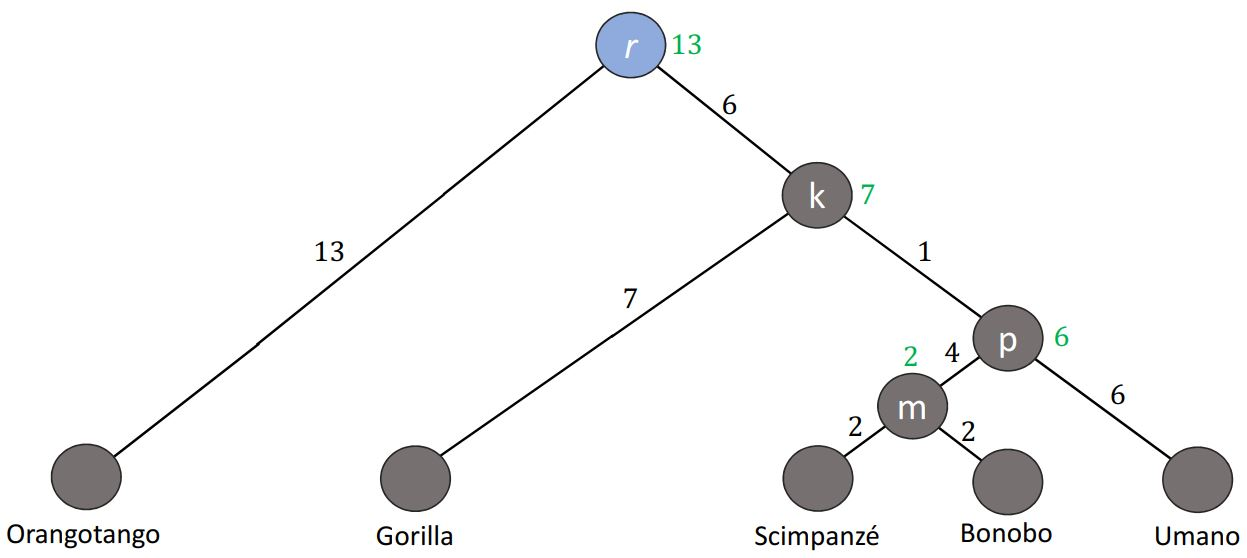
\includegraphics[height=15cm, width=13cm, keepaspectratio]{rooted_upgma_1.jpg}
 	\caption{Esempio di albero ultrametrico.}
  	\label{fig:rooted_upgma_1}
\end{figure}
\newline
In tale albero i nodi interni rappresentano la speciazione, ovvero quel processo attraverso il quale si forma una nuova specie. Questo significa che una singola linea evolutiva viene divisa in due \cite{speciationBritannica} e quindi un antenato sarà suddiviso in due discendenti. Si può notare che i numeri in verde accanto a tali nodi indicano l'età (in milioni di anni), mentre il peso degli archi è dato dalla differenza tra l'età dei nodi. ad esempio il pese dell'arco che collega $k$ e $p$ è dato dalla loro differenza ($7-6=1$). Poiché le foglie sono le specie  ancora non suddivise, la loro età è zero.
\newline
L'algoritmo \textit{UPGMA} può essere diviso in più fasi. Si prenda in considerazione la seguente matrice \textit{non additiva}\footnote{Per brevità si definisce u=umano, s=scimpanzé, f=foca, b=balena.}:
\[
D = \bordermatrix{\text{specie}&f&b&u&s\cr
                f& 0 & 3 & 4 & 3\cr
                b& 3 & 0 & 4 & 5\cr
                u& 4 & 4 & 0 & 2\cr
                s& 3 & 5 & 2 & 0}
\]
Si può notare che è la stessa matrice usata nella sezione dedicata al Neighbor-Joining.
\newline
\textit{Fase uno} $\rightarrow$ a partire da $D$ si formano $n$ cluster\footnote{Insiemi di elementi che condividono una determinata proprietà \cite{cambdrigeClusterDef}.}, ciascuno contenente una foglia, dove $n$ sono numero di righe (o colonne) della matrice.
\begin{figure}[h!]
\centering
	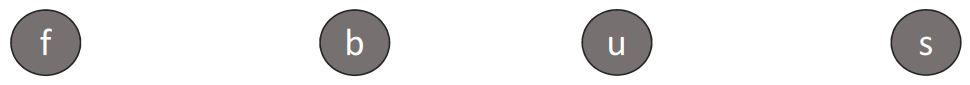
\includegraphics[height=1cm, width=12cm, keepaspectratio]{rooted_upgma_2.jpg}
 	\caption{Cluster iniziale.}
  	\label{fig:rooted_upgma_2}
\end{figure}
\newline
\textit{Fase due} $\rightarrow$ si scelgono i due cluster più vicini $X$ e $Y$ secondo la seguente definizione di distanza \cite{understandingBioinf}:
\[
D_{X,Y}=\frac{1}{\left | X \right |\cdot \left | Y \right |} \cdot \sum_{i\in X,\: j\in Y}D_{i,j}
\]
Dove $i$ sono gli elementi del cluster $X$, $j$ del cluster $Y$, $D_{i,j}$ è la distanza tra $i$ e $j$, $ \left | X \right | $ e $ \left | Y \right | $ sono rispettivamente il numero degli elementi in $X$ ed in $Y$. Poiché in questo caso  ciascun cluster è formato da un solo elemento, prendere i due cluster più vicini equivale a scegliere l'elemento più piccolo in $D$, ovvero $D_{u,s}$.
\newline
\textit{Fase tre} $\rightarrow$ si crea un cluster $Z$ che è dato dall'unione tra $X$ ed $Y$. Nel caso di $D$, il risultato di questo passo è il seguente:
\newpage
\begin{figure}[h!]
\centering
	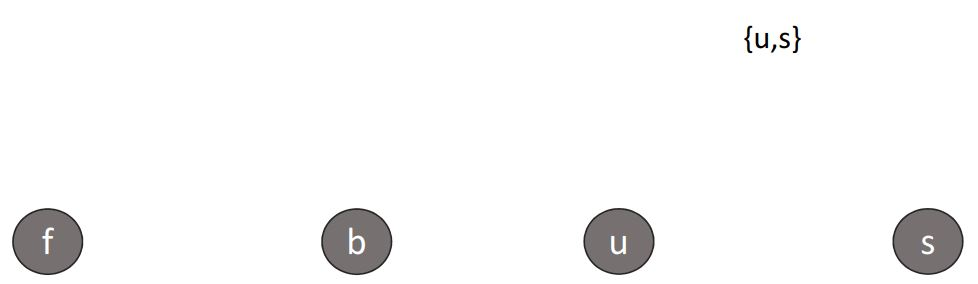
\includegraphics[height=6cm, width=9cm,keepaspectratio]{rooted_upgma_3.jpg}
 	\caption{Il cluster $\{u, s\}$ è stato ottenuto attraverso l'unione tra $u$ ed $s$.}
  	\label{fig:rooted_upgma_3}
\end{figure}
\textit{Fase quattro} $\rightarrow$ si forma un nodo interno per $Z$ la cui età è $age(Z)=\frac{D_{X,Y}}{2}$ e si calcola il peso degli archi\footnote{Come detto poc'anzi, il peso dell'arco che collega $Z$ ad $X$ è uguale alla differenza della loro età.}. Applicato all'esempio si ottiene che:
\[age(\{u, s\})=\frac{D_{u,s}}{2}=\frac{2}{2}=1\]
\[edgeweight(\{u, s\},s)=age(\{u, s\})-age(s)=1-0=0\]
\[edgeweight(\{u, s\},u)=age(\{u, s\})-age(u)=1-0=0\]
L'albero risultante è:
\begin{figure}[h!]
\centering
	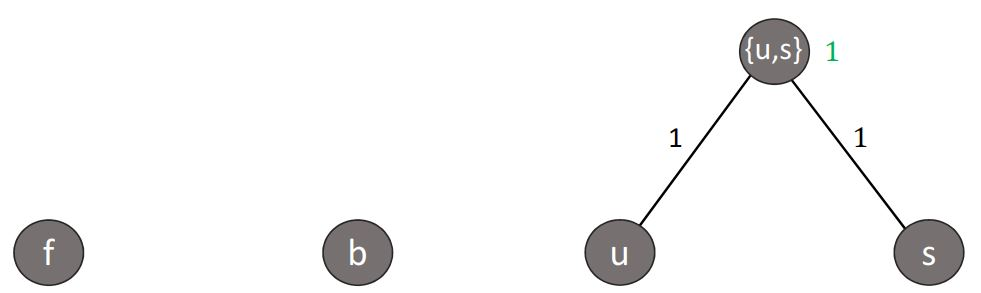
\includegraphics[height=9cm, width=11cm,keepaspectratio]{rooted_upgma_4.jpg}
 	\caption{Albero $T$ dopo aver calcolato l'età dei nodi ed il peso degli archi.}
  	\label{fig:rooted_upgma_4}
\end{figure}
\newline
\textit{Fase cinque} $\rightarrow$ Si aggiorna la matrice $D$ calcolando la distanza tra i cluster usando la formula $D_{X,Y}=\frac{1}{\left | X \right |\cdot \left | Y \right |} \cdot \sum_{i\in X,\: j\in Y}D_{i,j}$, che è quella usata nella fase due. Quindi:
\[
D = \bordermatrix{\text{specie}&f&b&\{u, s\}\cr
                f& 0 & 3 & {\color{Blue} 3,5}\cr
                b& 3 & 0 & {\color{Blue} 4,5}\cr
                \{u, s\}& {\color{Blue} 3,5} & {\color{Blue} 4,5} & 0}
\]
Dove i nuovi valori sono ottenuti da:
\[D_{f, \{u, s\}}=\frac{D_{f,u}+D_{f,s}}{2}=\frac{4+3}{2}=\frac{7}{2}=3,5\]
\[D_{b, \{u, s\}}=\frac{D_{b,u}+D_{b,s}}{2}=\frac{4+5}{2}=\frac{9}{2}=4,5\]
A questo punto vanno eseguite le cinque fasi sopraelencate fino a che non otteniamo un unico cluster contenente tutte le specie.
\newline
\textit{Fase uno, due e tre} $\rightarrow$  si formano $n$ cluster a partire dalla nuova matrice $D$, si sceglie l'elemento più piccolo (e quindi $D_{f, b}$) e si crea un cluster $\{f, b\}$ a partire da $f$ ed $b$, quindi:
\begin{figure}[h!]
\centering
	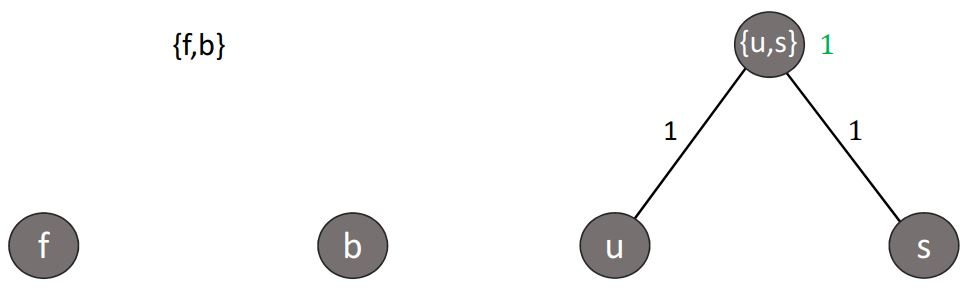
\includegraphics[height=6cm, width=9cm,keepaspectratio]{rooted_upgma_5.jpg}
 	\caption{Il cluster $\{f, b\}$ è stato ottenuto attraverso l'unione tra $f$ ed $b$.}
  	\label{fig:rooted_upgma_5}
\end{figure}
\newline 
\textit{Fase quattro} $\rightarrow$ si forma un nodo interno per il cluster $\{f, b\}$ e si calcola sia la sua età che il peso dei rispettivi archi, quindi:
\[age(\{f, b\})=\frac{D_{f,b}}{2}=\frac{3}{2}=1,5\]
\[edgeweight(\{f, b\},b)=age(\{f, b\})-age(b)=1,5-0=1,5\]
\[edgeweight(\{f, b\},f)=age(\{f, b\})-age(f)=1,5-0=1,5\]
L'albero risultante è:
\begin{figure}[h!]
\centering
	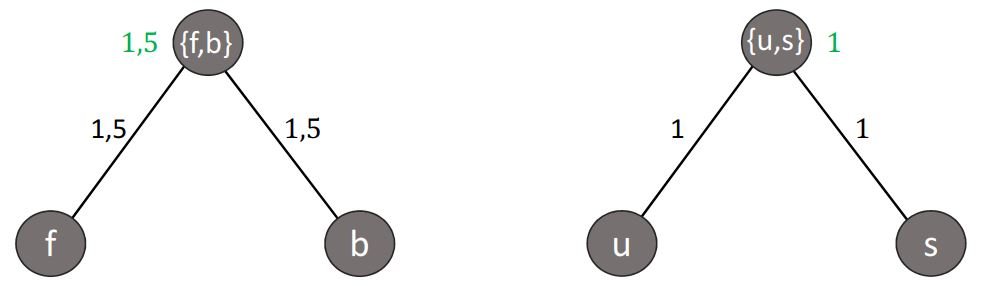
\includegraphics[height=9cm, width=11cm,keepaspectratio]{rooted_upgma_6.jpg}
 	\caption{Albero $T$ dopo aver calcolato l'età dei nodi ed il peso degli archi.}
  	\label{fig:rooted_upgma_6}
\end{figure}
\newline
\newline
\textit{Fase cinque} $\rightarrow$ Si aggiorna la matrice $D$ calcolando la distanza tra i cluster usando la formula $D_{X,Y}=\frac{1}{\left | X \right |\cdot \left | Y \right |} \cdot \sum_{i\in X,\: j\in Y}D_{i,j}$. La nuova matrice $D$ è:
\[
\
\]
Dove l'elemento $D_{\{f, b\}, \{u, s\}}$ è ottenuto da:
\[D_{\{f, b\}, \{u, s\}}=\frac{D_{f, \{u, s\}}+D_{b, \{u, s\}}}{2}=\frac{3,5+4,5}{2}=\frac{8}{2}=4\]
\newline
Si poiché ancora non abbiamo ottenuto un solo cluster, bisogna eseguire nuovamente gli step. Quindi si ha che:
\begin{itemize}
	\item l'elemento più piccolo è l'unico rimasto, ovvero $D_{\{f, b\}, \{u, s\}}$;
	\item si crea un nuovo cluster $\{f, b\}, \{u, s\}$ e si forma un nodo interno per esso, che sarà la radice dell'albero $T$. L'età è $age(\{f, b\}, \{u, s\})=\frac{D_{\{f, b\}, \{u, s\}}}{2}=\frac{4}{2}=2$, mentre gli archi sono $age(\{f, b\}, \{u, s\})-age(\{f, b\})=2-1,5=0$ e $age(\{f, b\}, \{u, s\})-age(\{u, s\})=2-1=1$. 
	\newline
	L'albero finale $T$ è:
	\begin{figure}[h!]
\centering
	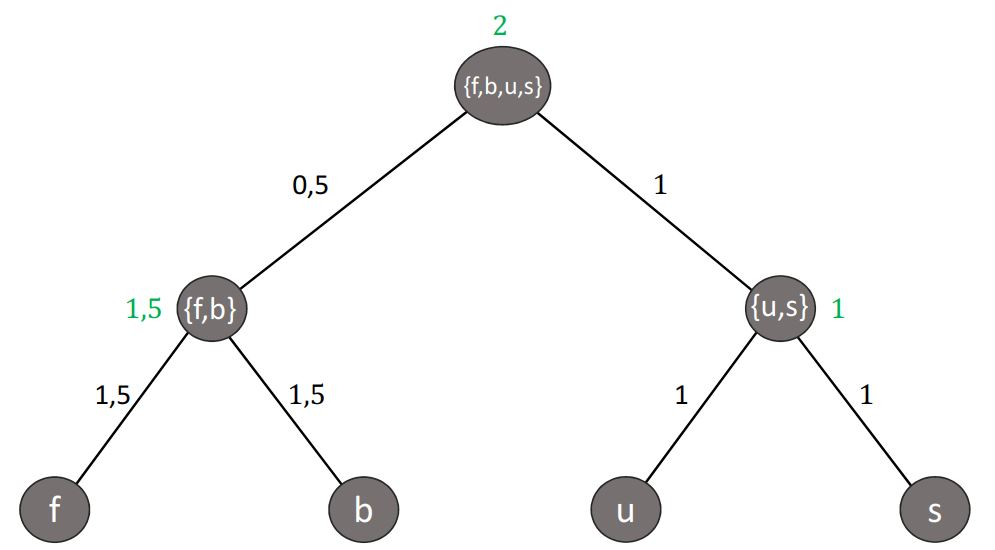
\includegraphics[height=12cm, width=14cm,keepaspectratio]{rooted_upgma_7.jpg}
 	\caption{Albero finale con radice $T$ ottenuto dalla matrice $D$.}
  	\label{fig:rooted_upgma_7}
  	\item si aggiorna la matrice $D$, ottenendo quindi:
  		\[
  		D = \bordermatrix{\text{specie}&\{f, b, u, s\}\cr
                \{f, b, u ,s\}& 2}
                \]
\end{figure}
\end{itemize}
Poiché abbiamo ottenuto l'abero $T$ e la matrice $D$ è composta da un unico cluster, l'algoritmo è terminato.